%\documentclass[12pt,letterpaper]{article}
%\usepackage{harvard}
%\usepackage{amsthm,amsfonts,amsmath}
%\usepackage{enumitem}
%%\usepackage[pdftex]{graphicx}%%for Pdftex
%\usepackage{graphicx}%%for Latex
%\usepackage{multirow}
%\usepackage{bbm}
%\usepackage{amssymb}
%\usepackage{amsthm}
%\usepackage{mathrsfs}
%
%%\usepackage[pdftex]{graphicx}
%%\usepackage{subfigure}
%%\usepackage{multicol}
%%\usepackage{color}
%\usepackage{algorithm}
%\usepackage{algorithmic}
%\usepackage{setspace}

\documentclass[12pt,letterpaper]{article}

\usepackage{hyperref}
\usepackage{harvard}
\usepackage{amsthm,amsfonts,amsmath}
\usepackage{enumitem}
%\usepackage[pdftex]{graphicx}%%for Pdftex
\usepackage{graphicx}%%for Latex
\usepackage{multirow}
\usepackage{bbm}
\usepackage{amssymb}
\usepackage{amsthm}
\usepackage{mathrsfs}
%\usepackage[pdftex]{graphicx}
%\usepackage{subfigure}
%\usepackage{multicol}
%\usepackage{color}
\usepackage{algorithm}
\usepackage{algorithmic}
\usepackage{setspace}


%%%%%%%%%%%%%%%%%%%%%%%%%%%%%%%%%%%%%%%%%%%%%%%%%%%%%%%%%%%%%%%%%%%%%%%%%
%                                                                       %
%                         Page settings                                 %
%                                                                       %
\topmargin -1.4cm %25pt         % 0 cm
    \headheight 2pt
    \headsep 20pt
\setlength{\textwidth}{16cm} \setlength{\textheight}{23cm}
\setlength{\oddsidemargin}{0.4cm} %   Left margin on odd-numbered pages. 0.9cm=>rand links=rand rechts
\setlength{\evensidemargin}{-2pt} %   Left margin on even-numbered pages.
\marginparwidth .875in
%\parskip 5pt plus 1pt %skip between paragraphs
\parindent 2em
\jot = 1.5ex \setlength{\footnotesep}{3pt}
\setlength{\unitlength}{1cm}

%%%%%%%%%%%%%%%%%%%%%%%%%%%%%%%%%%%%%%%%%%%%%%%%%%%%%%%%%%%%%%%%%%%%%%%%%
\hyphenation{con-tin-u-ous-time con-tin-u-ous bank-rupt-cy}
\hyphenation{Lebes-gue} \hyphenation{ter-mi-nol-o-gy}
%%%%%%%%%%%%%%%%%%%%%%%%%%%%%%%%%%%%%%%%%%%%%%%%%%%%%%%%%%%%%%%%%%%%%%%%%
\newcommand{\bbr}{\mathbb{R}}  %black board bold \mathbb{R}
\newcommand{\bbn}{\mathbb{N}}
\newcommand{\bbp}{\mathbb{P}}
\newcommand{\bY}{\mathbf{Y}}
\newcommand{\mun}{\lceil \mu n \rceil}
\newcommand{\etan}{\lceil \eta n \rceil}
\newcommand{\bbq}{\mathbb{Q}}
\newcommand{\wQ}{\widetilde{\bbp}}%change per Prof. Lai's request to alleviate confusion
\newcommand{\wq}{\widetilde{p}}%change per Prof. Lai's request to alleviate confusion
\newcommand{\wY}{\widetilde{Y}}
\newcommand{\ow}{\overline{w}}
\newcommand{\wht}{\widehat}
\newcommand{\var}{\ensuremath{\mathbb Var}}
\newcommand{\wbY}{\widetilde{\bY}}
\newcommand{\abs}[1]{\lvert#1\rvert}
\newcommand{\D}{\mathbb{D}}
\newcommand{\G}{\mathbb{G}}
\newcommand{\bbe}{\mathbb{E}}
\newcommand{\F}{\mathbb{F}}
\newcommand{\HH}{\mathbb{H}}
\newcommand{\bbj}{\mathbb{J}}
\newcommand{\bbz}{\mathbb{Z}}
\newcommand{\bbs}{\mathbb{S}}
\newcommand{\C}{\mathbb{C}}
\newcommand{\bu}{\mathbf{u}}
\newcommand{\bx}{\mathbf{x}}
\newcommand{\fn}{\footnote}
\newcommand{\ci}{\citeasnoun}
\newcommand{\om}{\omega}
\newcommand{\la}{\lambda}
\newcommand{\tla}{\tilde{\lambda}}
\newcommand{\doth}{f}
\renewcommand{\labelenumi}{\roman{enumi}}
\newcommand{\ps}{P}
\newcommand{\pss}{\ensuremath{\mathbf{p}}} %small boldface
\newcommand{\pmq}{\ensuremath{\mathbf{Q}}}
\newcommand{\pmqs}{\ensuremath{\mathbf{q}}}
\newcommand{\pas}{P-a.s. }
\newcommand{\pasm}{P\mbox{-a.s. }}
\newcommand{\asm}{\quad\mbox{a.s. }}
\newcommand{\cadlag}{c\`adl\`ag }
\newcommand{\fil}{\mathcal{F}}
\newcommand{\gcal}{\mathcal{G}}
\newcommand{\hcal}{\mathcal{H}}
\newcommand{\jcal}{\mathcal{J}}
\newcommand{\pcal}{\mathcal{P}}
\newcommand{\ecal}{\mathcal{E}}
\newcommand{\bcal}{\mathcal{B}}
\newcommand{\ical}{\mathcal{I}}
\newcommand{\scal}{\mathcal{S}}
\newcommand{\ncal}{\mathcal{N}}
\newcommand{\lcal}{\mathcal{L}}
\newcommand{\kcal}{\mathcal{K}}
\newcommand{\acal}{\mathcal{A}}
\newcommand{\mcal}{\mathcal{M}}
\newcommand{\rcal}{\mathcal{R}}
\newcommand{\tcal}{\mathcal{T}}
\newcommand{\ti}{\times}
\newcommand{\we}{\wedge}
\newcommand{\be}{\begin{equation}}
\newcommand{\ee}{\end{equation}}
\newcommand{\bew}{\begin{equation*}}
\newcommand{\eew}{\end{equation*}}
\newcommand{\uK}{\underline K}
\newcommand{\oK}{\overline K}
\renewcommand{\th}{\tilde{h}}
\newcommand{\imp}{\eta}
\newcommand{\xbar}{\overline{X}}
\newcommand{\Xij}{X_{i,j}}
\newcommand{\f}{\left}
\newcommand{\g}{\right}
\newcommand{\naiveest}{\wht{\sigma^2_n}}
\newcommand{\deltaest}{\wht{\sigma^2_d}}

\setcounter{topnumber}{1}
\setcounter{totalnumber}{1}


\newtheorem{thm}{Theorem}
\newtheorem{cond}[thm]{Condition}
\newtheorem{defi}[thm]{Definition}
\newtheorem{algo}[thm]{Algorithm}
\newtheorem{prop}[thm]{Proposition}
\newtheorem{corollary}[thm]{Corollary}
\newtheorem{lem}[thm]{Lemma}
\newtheorem{rem}[thm]{Remark}
\newtheorem{ex}[thm]{Example}
\newtheorem{ass}[thm]{Assumption}

\frenchspacing

%*******************************************************************************
%*******************************************************************************



\begin{document}
\renewcommand{\labelenumi}{\arabic{enumi}.}
\renewcommand{\baselinestretch}{1.05} \small \normalsize
\title{True Variance of Non-user Level Metrics}
\author{Shaojie Deng}
\date{4/4, 2011\\ This version: \today}
\maketitle
\part{Randomization by User}
\section{Notation}
Denote $n$ the number of unique users. Denote $X_{i,j}$ the per-page measurement on user $i$'s $j^{th}$ page view and $X_{i,j}$ has mean $\mu_i$ and variance $\sigma_i^2$ (i.e., means and variances are different from user to user). Denote $K_i$ the total number of page views from user $i$ and $N = \sum_{i=1}^n K_i$ be the total number of page views.   

Using preceding notation, the page level metric can be denoted by:
\begin{align}
\xbar= \frac{\sum_{i=1}^n\sum_{j=1}^{K_i} X_{i,j}}{N}
\end{align}

If we treat page veiw level metrics $X_{i,j}$ as i.i.d., the naive estimator for the variance of $\overline{X}$ is:
\begin{align}
\frac{1}{N^2} \Bigl (\sum_{i=1}^n \sum_{j=1}^{K_i} (X_{i,j}-\overline{X})^2 \Bigr )
\end{align}
For asymptotic analysis, we will let $n\to \infty$ (so $N\to \infty$ a.s.) and threfore we need to normalize the estimator by $n$.  We introduce the normalized estimator 
\begin{align}
\wht{\sigma^2_n} = n\frac{1}{N^2} \Bigl (\sum_{i=1}^n \sum_{j=1}^{K_i} (X_{i,j}-\overline{X})^2 \Bigr )
\end{align}

If we treat user level metrics $(\sum_{i=1}^{K_i} \Xij , K_i)$ as i.i.d,  we can use the delta method to estimate the normalized variance $n\var \xbar$. We denote it by $\wht{\sigma^2_d}$. 
In the following, we will investigate what is the true value of $n\var \xbar$ and what is the bias factor of using naive estimator $\naiveest$. In the next section, we will consider the case where we assume we have infinite users and we sample from the pool with replacement, i.e., users are sampled i.i.d. 
In Section \ref{finitecase}, we will consider the case that we have in total $M$ users and we sample $x\%$ of users from that finite pool of users without replacement. This case is more realistic but it reduce to the i.i.d. case when $x$ is close to 0. In all cases, we assume $K_i$ and $(\mu_i, \sigma^2_i)$ are independent. For technical reason, we also impose regularity conditions that $\mu_i$ and $\sigma^2_i$ are bounded above by a finite constant. 

\section{Infinte user pool case}\label{infcase}
By conditional variance formula, 
\begin{align}
&\var \xbar = \var \Bigl( \frac{\sum_{i=1}^n\sum_{j=1}^{K_i} X_{i,j}}{N} \Bigr) \notag \\
 =& \var  \Bigl( \bbe\Bigl(   \frac{\sum_{i=1}^n\sum_{j=1}^{K_i} X_{i,j}}{N} \Big| K_i,\mu_i,\sigma_i^2,  i=1,\dots,n\Bigr) \Bigr) \\
+&\bbe \Bigl(\var \Bigl( \frac{\sum_{i=1}^n\sum_{j=1}^{K_i} X_{i,j}}{N} \Big | K_i,\mu_i,\sigma_i^2,  i=1,\dots,n\Bigr)\Bigr) \notag\\
=&\var \Bigl(\frac{1}{N}\sum_{i=1}^n K_i \mu_i \Bigr)+\bbe \Bigl(\frac{1}{N^2}\sum_{i=1}^n K_i \sigma^2_i \Bigr)  \label{basicformula}
\end{align}

Using \eqref{basicformula}, we are interested in the limit of the normalized variance 
\[n \var \xbar = n\var \Bigl(\frac{1}{N}\sum_{i=1}^n K_i \mu_i \Bigr)+n\bbe \Bigl(\frac{1}{N^2}\sum_{i=1}^n K_i \sigma^2_i \Bigr) \text{ as } n\to \infty.\]
Let $w_i = K_i/\sum_{i=1}^n K_i = K_i/N$. Since $K_i$ independent of $(\mu_i, \sigma^2_i)$ and $N/n \to \bbe {K_i}$ as $n\to \infty$, we can further simplify the right hand. First, by applying iterative expectation(frist conditioning on $w_1,\dots, w_n$), we have  
\begin{align}
n \bbe \Bigl(\frac{1}{N^2}\sum_{i=1}^n K_i \sigma^2_i \Bigr)  = \sum_{i=1}^n \bbe\Bigl( \frac{n}{N} w_i\sigma^2_i \Bigr) = \frac{1}{\bbe K_i}(\sum_{i=1}^n w_i)\bbe \sigma_i^2 = \frac{\bbe \sigma_i^2}{\bbe K_i} \label{withinterm}
\end{align}
where the second equality is by bounded convergence theorm(since $N/n \to \bbe {K_i}$ and $\sum w_i\sigma^2_i$ bounded) and the last equation is from $\sum w_i=1$. 
Next, since $(\mu_i, \sigma^2_i)_{i=1,\dots, n}$ are i.i.d., 
\begin{align}
&n\var (\sum_{i=1}^n w_i \mu_i) = n\bbe (\var (\sum_{i=1}^n w_i \mu_i|w_1,\dots,w_n))+ n\var (\bbe (\sum_{i=1}^n w_i \mu_i|w_1,\dots,w_n)) \\
&=  n\bbe (\sum_{i=1}^n w_i^2 \var(\mu_i)) + n \var((\sum_{i=1}^n w_i)\bbe\mu_i ) = n\bbe(\sum_{i=1}^n w_i^2) \var (\mu_i) \label {betweenterm}
\end{align}
since the second term is $0$.

We've reached the following proposition:
\begin{prop}\label{prop1}
If there exists a constant $C>0$ such that $n\bbe(\sum_{i=1}^n w_i^2)\to C$, then under the previous assumptions, 
\begin{align}
 n\var\xbar \to C \var(\mu_i) + \bbe(\sigma^2_i)/\bbe (K_i) 
\end{align}
\end{prop}

\begin{rem}
When $\var \mu_i =0$, i.e., there is no between user variation. $ n\var\xbar \to \bbe(\sigma^2_i)/\bbe (K_i) $.
\end{rem}

We now calculate the expectation of $\naiveest$. 
\begin{align*}
\bbe \naiveest &= n \bbe\Bigl( \frac{1}{N^2} \Bigl (\sum_{i=1}^n \sum_{j=1}^{K_i} (X_{i,j}-\overline{X})^2 \Bigr )\Bigr) = n\bbe \Bigl \{  \sum_{i=1}^n \sum_{j=1}^{K_i} (X_{i,j}^2 - N \xbar^2  \Bigr\}\\
&= \bbe \Bigl( \frac{n^2}{N^2}  \sum_{j=1}^{K_i} \Xij^2  \Bigr) - \bbe \Bigl( \frac{n}{N}  \xbar^2  \Bigr) \quad \text{since $\sum_{j=1}^{K_i}\Xij^2$ identically distributed for all $i$}\\ 
\end{align*}
Using bounded convergence theroem and $N/n \to \bbe K_i$, the first term converges to 
\[
1/\bbe(K_i)^2 \times \bbe(K_i) \bbe(\Xij^2) = (\bbe(\sigma_i^2)+\bbe(\mu_i^2) )/\bbe(K_i).
\]
For the second term, similarly by bounded convergence theorem, 
\[\bbe \bigl((n/N) \xbar^2\bigr) \to \bbe(\xbar^2)/\bbe(K_i).\] 
Note that 
\begin{align*}
\bbe (\xbar^2) = \var(\xbar)+ \bbe^2 (\xbar)  \to \bbe^2(\xbar)  \quad \text{since $\var(\xbar) \to 0$ as $n\to \infty$}.
\end{align*}
Also, 
\begin{align*}
\bbe \xbar= \bbe \Bigl( \frac{n}{N} \sum_{j=1}^{K_i} \Xij \Bigr) \to \bbe(\Xij) = \bbe(\mu_i) . 
\end{align*} 
It is straightforward combination of these two results that we have proved: 
\begin{prop}\label{prop2}
Under these conditions, as $n\to \infty$
\begin{align}
\bbe(\naiveest) \to  \frac{1}{\bbe(K_i)} (\var(\mu_i)+\bbe(\sigma_i^2))
\end{align}
\end{prop}

Now we can state the main theorem for this section:
\begin{thm}[Bias Factor]\label{thm1}
Under the conditions of Proposition \ref{prop1} and \ref{prop2}, as $n\to \infty$, 
\begin{align}
\frac{n\var (\xbar)}{\bbe(\naiveest)} \to  (\bbe(K_i)C - 1)\rho +1
\end{align}
where $\rho:= \var(\mu_i)/(\var(\mu_i)+\bbe(\sigma^2_i))$ is the user effect coefficient(variances that explained by between user variation). 
\end{thm}

\begin{rem}
When $K_i \equiv K, i=1,\dots, n$, $C=1$ and the ratio in \label{thm1} becomes $(K-1)\rho +1$. This recovers Susan's formula.  
\end{rem}

Finally, it is a known result that delta method estimator $\deltaest$ provides asymptotically unbiased estimators for $n\var(\xbar)$  under the assumption that users are i.i.d., which is true under the conditions of this section. We have the following proposition:
\begin{prop}\label{prop-delta}
If there exists a constant $C>0$ such that $n\bbe(\sum_{i=1}^n w_i^2)\to C$, then under the previous assumptions, 
\begin{align}
\bbe (\deltaest) \to C \var(\mu_i) + \bbe(\sigma^2_i)/\bbe (K_i) .
\end{align}
\end{prop}

As a final remark, all the results in this section relies on the assumption that there exists a constant $C>0$ such that $n\bbe(\sum_{i=1}^n w_i^2)\to C$. We now prove that this is the case.
\begin{prop}\label{prop0}
As $n\to\infty$, $n\bbe(\sum_{i=1}^n w_i^2)\to \frac{\bbe K_i^2}{(\bbe K_i)^2}$. Moreover, $C = \frac{\bbe K_i^2}{(\bbe K_i)^2} \ge 1$ with the equality only attained when $K_i$ is constant.
\end{prop}
\begin{proof}
We prove $n \sum_{i=1}^n w_i^2 \to  \frac{\bbe K_i^2}{(\bbe K_i)^2}$ a.s. To see this, 
\begin{align*}
n \sum_{i=1}^n w_i^2 =  \frac{\overline{K_i^2}}{\overline{K_i} \times \overline{K_i}}
\end{align*}
By strong law of large number, $\overline{K_i^2}\to \bbe K_i^2$ a.s., $\overline{K_i}\to \bbe K_i$ a.s., therefore $n \sum_{i=1}^n w_i^2 =  \frac{\bbe{K_i^2}}{(\bbe{K_i})^2}$ a.s. and the results follows. 

By Jensen's inequality and convexity of the function $x^2$, $\bbe K_i^2 \ge (\bbe K_i)^2$ with the equality attained if and only if $K_i$ constant. 
\end{proof}

\section{Finite user pool case}\label{finitecase}
In this section, we consider a more realistic model. Suppose we only have finite number of users, though the number can be very large. We label these users by index $i=1,\dots, M$ and suppose they have their own $(\mu_i,\sigma_i^2)$ fixed. 
For the experiment, we sampled a portion $x$ of users from the $M$ total users without replacement where $0<x\le 1$.  wlog, in the following we let $n = xM$ and treat it as an integer. Note that because users are sampled without replacement, they are no longer i.i.d. 
The goal of this section is to get similar result in Theorem \ref{thm1} under this dependent framework. For simplicity of notation, I suppose we first shuffle the $(\mu_i,\sigma^2_i)_{i=1,\dots,M}$ and then relabel these from $1$ to $M$. We then select the first $i=1,\dots,xM$  as the users that we sampled.\footnote{The purpose of using this model is that we can still use index $i=1,\dots,n$ in the proof rarther than introducing an additional layer of index $S_i$ denoting the index of the $i^{th}$selected user. } 

\begin{prop}\label{prop3}
If there exists a constant $C>0$ such that $n\bbe(\sum_{i=1}^n w_i^2)\to C$, then under the assumptions of this section, for any fixed $x$, as $n\to \infty, M\to \infty$ and $n/M = x$
\begin{align}
 n\var\xbar \to (C-x) \var(\mu_i) + \bbe(\sigma^2_i)/\bbe (K_i) 
\end{align}
\end{prop}

\begin{proof}
Note that \eqref{basicformula} is still true under the new model. The second term of \eqref{basicformula} is in the form of an expectation, which is a linear operator so dependencies among $\sigma_i^2$ doesn't really matter. Therefore the second term is equal to $\bbe(\sigma_i^2)/\bbe(K_i)$, the same as the second term in Proposition \ref{prop1}. 
For the first term, 
\begin{align*}
n\var (\sum_{i=1}^n w_i \mu_i) &= n\bbe (\sum_{i=1}^n w_i \mu_i| w_1,\dots w_n) + n\var( \bbe(\mu_i)\sum_{i=1}^n w_i)\\
&  =  n\bbe \bigl(\var(\sum_{i=1}^n w_i \mu_i| w_1,\dots w_n) \bigr).
\end{align*}
Since now $\mu_i$ are not independent, we need to consider their covariances:
\begin{align*}
&\var(\sum_{i=1}^n w_i \mu_i| w_1,\dots w_n) = \sum_{i=1}^nw_i^2 \var(\mu_i) + \sum_{i\neq j} w_i w_j Cov(\mu_i,\mu_j).
\end{align*}
It is trivial that $\var \bigl((\sum_{i=1}^n w_i)^2\bigr) =0$ because $\sum w_i =1$. 
\begin{align*}
0 = \var \bigl((\sum_{i=1}^n w_i)^2\bigr) = \sum_{i=1}^n \var(w_i) + \sum_{i\neq j} Cov(w_i,w_j). 
\end{align*}
Hence $Cov(w_i,w_j)=-\var(w_i)/n$.

Similarly $\var(\sum_{i=0}^M \mu_i) = 0$ since $\sum_{i=1}^M \mu_i$ is invariant against shuffling, and the same argument implies $Cov(\mu_i,\mu_j) = - \var(\mu_i)/M$ . 
\begin{align*}
&n\bbe \bigl(\var(\sum_{i=1}^n w_i \mu_i| w_1,\dots w_n) \bigr)= n\bbe(\sum_{i=1}^nw_i^2)\var(\mu_i) + n \sum_{i\neq j} \bbe(w_i w_j) Cov(\mu_i,\mu_j)\\
&= n\bbe(\sum_{i=1}^nw_i^2)\var(\mu_i) + n\times n(n-1)\bbe(w_i w_j) (-\var(\mu_i)/M) 
\end{align*}
The first term converges to $C \var(\mu_i)$. For the second term, 
\begin{align*}
&n\times n(n-1)\bbe(w_i w_j) (-\var(\mu_i)/M) = n\times n(n-1)(\bbe^2(w_i)+Cov(w_i,w_j)) (-\var(\mu_i)/M)\\
&= n\times n(n-1)(\frac{1}{n^2}-\var(w_i)/n)(-\var(\mu_i)/M)\to - x \var (\mu_i)
\end{align*}
where the last step uses the fact that $n\var(w_i)\le n\bbe(w_i^2)\to 0$ under the assumption $n\bbe(\sum_{i=1}^nw_i^2)\to C<\infty$.

Combining pieces together, we have proved the proposition.
\end{proof}

A closer look of the proof of Proposition \ref{prop2} reveals it never used the $(\mu_i,\sigma_i^2)$ i.i.d. assumption. So it is still true even under the framework of this section. 
\begin{prop}\label{prop4}
Under the assumptions of this section, for any fixed $x$, as $n\to \infty, M\to \infty$ and $n/M = x$
\begin{align}
\bbe(\naiveest) \to  \frac{1}{\bbe(K_i)} (\var(\mu_i)+\bbe(\sigma_i^2))
\end{align}
\end{prop}

Now let us think about the delta method. Delta method is based on the assumption that users are i.i.d. Therefore, if we apply delta method, i.e., use $\deltaest$ to estimate $n\var(\xbar)$, it will converge to the same value under the condition in Section \ref{infcase}, which is $C\var(\mu_i) + \bbe(\sigma^2_i)/\bbe (K_i)$. 

Combining all the previous results in this section, we have proved the following theorem:
\begin{thm}[Formula X]\label{thm-2}
Under the assumptions in this section, for any fixed $x$, as $n\to \infty, M\to \infty$ and $n/M = x$
\begin{align}
 n\var\xbar &\to (C-x) \var(\mu_i) + \bbe(\sigma^2_i)/\bbe (K_i), \\
\bbe(\naiveest)&\to   \frac{1}{\bbe(K_i)} (\var(\mu_i)+\bbe(\sigma_i^2)),\\
\bbe(\deltaest)&\to C\var(\mu_i) + \bbe(\sigma^2_i)/\bbe (K_i)
\end{align}
In practice we will be able to compute $\naiveest$ and $\deltaest$, we can also estimate $\bbe(K_i)$ by $\wht{\bbe{K_i}}=\overline{K_i}$ and $C$ by $\wht{C}=n^2\overline{w_i^2}$, therefore the true variance $n\var\xbar$ can be estimated by:
\begin{align}\label{formula}
\wht{n\var(\xbar)} = \deltaest - x \frac{\deltaest-\naiveest}{\wht{C}-1/\wht{\bbe(K_i)}}.\tag{Formula X}
\end{align}
\end{thm}


\section{Simulation Study}\label{simstudy}
In this simulation study, we prescribed $M=1,000,000$ number of users. Each of them have a fixed click through rate $p_i$ and we generate these $M$ $p_i$ from a $Beta(0.1,0.5)$ distribution. Figure~\ref{fig:beta-dist} shows the shape of this distribution. Once these $p_i$'s are sampled, they will be fixed through out the whole simulation study. 
\begin{figure}[!hbtp]
  \centering
  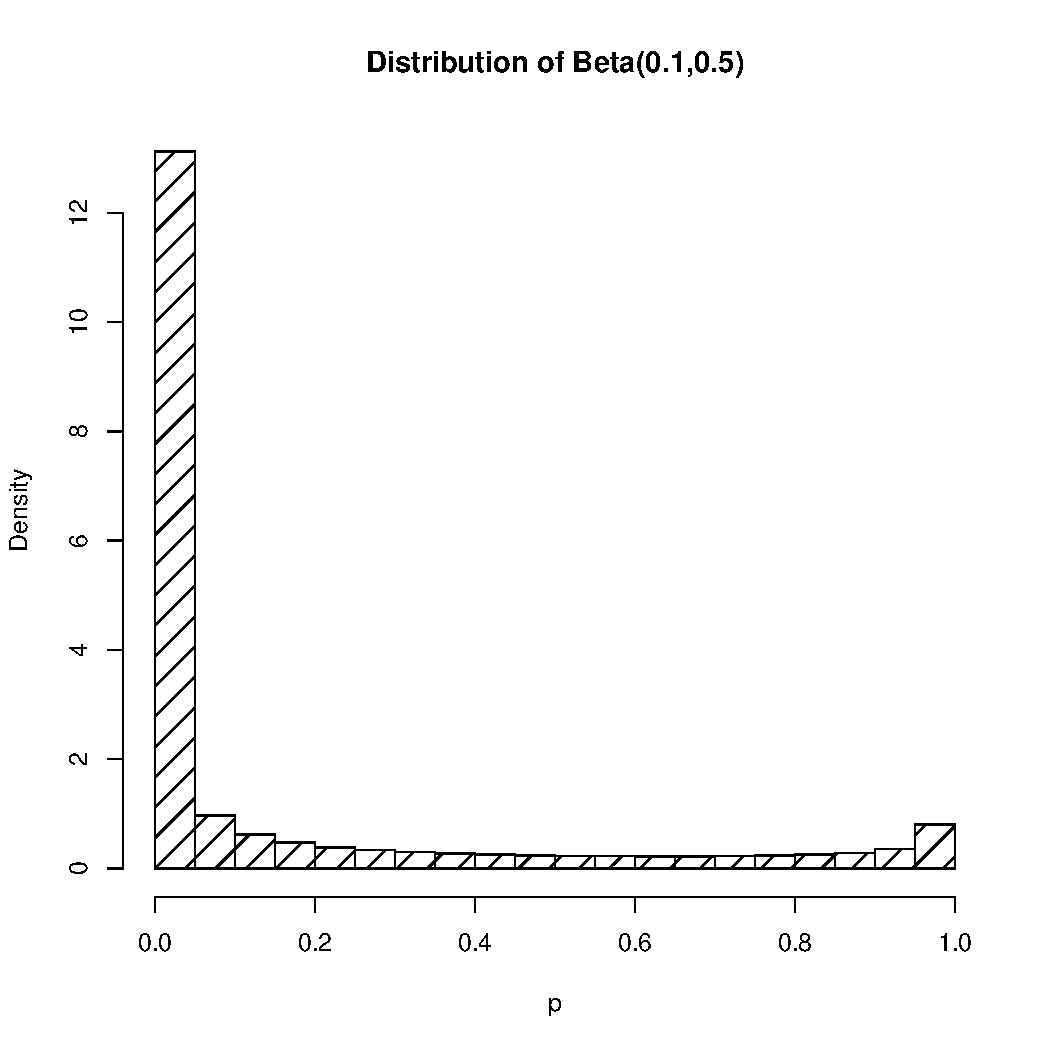
\includegraphics[width=.5\textwidth]{beta-dist}
  \caption{The distribution of users' click trough rate parameter $p_i$ from $Beta(0.1,0.5)$ distribution.}
  \label{fig:beta-dist}
\end{figure}
For the step 2,  each time, we sample a proportion $x$ of users as well as their $p_i$ from the $M$ users without replacement. Then we simulate the page view $K_i$ for each selected users from 
$Poisson(6)$ and we add $1$ to make it nonzero(Actually this is not necessary, will Do it again without adding 1). The rest of the simulation is straightforward, we simulate the number of click through for user $i$ from $Binomial(K_i,p_i)$. We then compute PCR, $\naiveest$ and $\deltaest$. To calculate the true variance, we repeat this step for $1000$ times and calculate sample variances of the PCR and take average of those $1000$ $\naiveest$ and $\deltaest$. 

The last step is to repeat Step 2 for a grid of $x$ from $0$ to $1$. We started with $x=0.02$ and linearly grow $x$ to $1$ with step size $0.02$. After this step, we normalized the 3 variances calculated by $n = xM$ and apply \eqref{formula}. The results are summarized in Figure~\ref{fig:ctr-poisK} 

\begin{figure}[!hbtp]
  \centering
  \includegraphics[width=0.9\textwidth]{ctr-poisK}
  \caption{Plot of 3 estimators for normalized variances(naive method, delta method, Formula X) and the estimated true variances. The formula X predicts linearly decreasing variances as $x$ increase from $0$ to $1$.}
  \label{fig:ctr-poisK}
\end{figure}

\section{Implications on on-line controlled experimentation}\label{implication}
The findings in both Section~\ref{infcase} and Section~\ref{finitecase} have obvious implications on on-line controlled experimentation. The results in Section~\ref{infcase} explains why treating page-view level measurements as independent underestimates the variance and quantified the bias factor. This topic has been covered in the non-user level metrics documents drafted by Ya and in this paper we treat the proof with more rigor and slightly changed the results.  

The implication of the results in Section~\ref{finitecase} is more subtle. For general controlled experiments, it is a natural and general practice to assume an infinite pool of users and based on this very assumption people treat users as independent even though we know each individual is a unique human being. We seldom questioned this practice because : First, delta method will only over-estimate the variance as \ref{formula} shows the true variance is always smaller than the delta method estimate. The type-I error will still get controlled. Second, when $x$ is close to 0, true variance and the delta method(or corresponding bootstrap estimates) are very close. So there is little gain of statistical power to actually use \ref{formula} for the calculation of variance.

 But things can be different for online controlled experiment. There is no limit stopping us from doing an A/B test with 50\% and 50\% users for control and treatment. These are usually the case when total traffic is low, i.e. Mobile. or the cases that we want to finish the experiment in a short time. For $x=0.5$, the effect of using \ref{formula} can really increase the power. For example, in the simulation study in Section \ref{simstudy}, the normalized delta method variance is about 0.105 and the normalized naive estimates is about 0.020. When $x=0.5$, the true variance was estimated to be $0.060$ and \ref{formula} gave $0.061$.
The true variance is about $57\%$ of the delta method estimate. How will this affect the statistical power?

If we assume the coefficient of variation(ratio of standard deviation to the mean) of the metric being flat against the length of the experiment. There is a simple approximated relationship between power $\beta$, Type-I error $\alpha$, the expected percentage change (treatment effect) $\delta\%$ and the sample size $n_1$ and $n_2$ of two groups:
\begin{align}\label{power}
\frac{1}{1/n_1+1/n_2}= cv^2\Bigl(\frac{\Phi_{\alpha/2}+\Phi_\beta}{\delta\%}\Bigr)^2
\end{align}  
Assuming $n_1=n_2=n$ and $\delta\%$ fixed and $cv$ remains flat as $n$ grows. Simple algebra on \eqref{power} reveals a decrease of variance from 1 to 0.57 is equivalent to increase n by $1/0.57=1.75$. Assuming $n$ grows linearly, the above derivaition suggests using \ref{formula} can reduce the experiment time by  a factor of $1.75$ and yet achieve the same power. In reality $n$ grows sublinearly and it is safe to say that the time reduced is more than a factor of $2$(To do: use empirical data). 


\part{Randomization by Page View}
\section{A two layer randomization framework}
Now we consider the case that randomization is done by page view. Suppose ALL page views are randomly divided into different groups. By ALL page views we mean page views from all users in the universe. Under this framework, it is from the typical marginalization argument that we can treat page view level measurement as i.i.d. i.e., there is no user effect in the analysis because the page views are drawn from all users and no user selection variance is induced in this randomization scheme. Since page view level measurements are i.i.d., all statistical analysis no finer than page view level is therefore straightforward. 

The case that is of more interest is the following. We do not want to perform experiment on all users. Instead, we first randomly selected $n$ user from all the users in the universe. $n$ is usually only a small percentage of the total number $M$ of users in the universe so let us assume $M$ is infinity and hence the users are drawn independently. All the page views from these $n$ users are then randomly split into control and treatment. The goal is to make inference by comparing some metrics in control and treatment. 

We inherit all the notations from Part I. Suppose we are interested in page view level metrics $\xbar_r = \sum_{i=1}^n \sum_{j=1}^{{K_i}^{(r)}}X_{i,j}^{(r)}/N_r$ where $r=1,2$ stands for control and treatment. In Part I, we never consider the variance of both control and treatment together. This is because the control and treatment groups have different users and since randomization is based on user, the metrics of the two groups are therefore independent. As a result the variance of the metrics difference is simply the sum of the two variances of metric in each group.  What make things more complicated is that the current framework, control and treatment share the same group of $n$ users. It is the page view, not the user that is randomized into two groups. Due to this very fact, $\xbar_1$ and $\xbar_2$ are no longer independent. 


\section{Variance formula}
In this section we give the asymptotically unbiased estimator for $\var (\xbar_1-\xbar_2)$ when the page views are split into control and treatment with fixed weights. For simplicity, we first assume control and treatment have the same weights. But we will give the result for general case in the end of this Section. Under the same assumption as in Part I that number of page views $K_i$ are independent of $(\mu_i,\sigma_i^2)$. Then conditioned on $K_i$, $K_i^{r}$ follows from $binomial(K_i, 0.5)$ distribution. If we only consider one group, say control. Then the only difference between this framework and that of Section \ref{infcase} is that now $K_i^{r}$ follows from a different distribution(from $K_i$). But note that all the result in Section \ref{infcase} does not depend on the distribution of $K_i$. Therefore all results in Section \ref{infcase} directly apply on $\xbar_1$ (or $\xbar_2$). 

\begin{prop}\label{p_prop1}
Let $w_i^{(r)}=K_i^{(r)}/\sum_{i=1}^{n} K_i^{(r)} $. Assume $n\bbe (\sum_{i=1}^n {(w_i^{(r)})}^2)\to C$, $r=1,2$ as $n\to \infty$. Then for $r=1,2$
\begin{align}
\bbe(\naiveest_r) &\to  \frac{1}{\bbe(K_i^{(r)})} (\var(\mu_i)+\bbe(\sigma_i^2)) \label{p_naive}\\
\bbe (\deltaest_r) &\to C \var(\mu_i) + \bbe(\sigma^2_i)/\bbe (K_i^{(r)}) \label{p_delta}.
\end{align}
\end{prop}

What Proposition \ref{p_prop1} says is exactly that if we apply naive formula or delta method formula to one group, we will get asymptotically unbiased estimator for the right hand side of \eqref{p_naive} and \eqref{p_delta}, respectively. 

To analyze $\var (\xbar_1-\xbar_2)$, we begin by using the basic formula \eqref{basicformula}, with  a little bit modification. 
\begin{align}
&\var (\xbar_1-\xbar_2) = \var \Bigl( \frac{\sum_{i=1}^n\sum_{j=1}^{K_i^{(1)}} X_{i,j}^{(1)}}{N_1} -\frac{\sum_{i=1}^n\sum_{j=1}^{K_i^{(2)}} X_{i,j}^{(2)}}{N_2}\Bigr) \notag \\
 =& \var \Bigl( \bbe \Bigl( \frac{\sum_{i=1}^n\sum_{j=1}^{K_i^{(1)}} X_{i,j}^{(1)}}{N_1} -\frac{\sum_{i=1}^n\sum_{j=1}^{K_i^{(2)}} X_{i,j}^{(2)}}{N_2}|K_i^{(r)}, \mu_i^{(r)},\sigma_i^{(r)},i=1,\dots,n, r=1,2) \Bigr)\Bigr)\notag \\
+&\bbe \Bigl(\var \Bigl( \frac{\sum_{i=1}^n\sum_{j=1}^{K_i^{(1)}} X_{i,j}^{(1)}}{N_1^2} -\frac{\sum_{i=1}^n\sum_{j=1}^{K_i^{(2)}} X_{i,j}^{(2)}}{N_2^2}|K_i^{(r)}, \mu_i^{(r)},\sigma_i^{(r)},i=1,\dots,n, r=1,2\Bigr)\Bigr) \notag\\
=&\var \Bigl(\frac{1}{N_1}\sum_{i=1}^n K_i^{(1)} \mu_i  - \frac{1}{N_2}\sum_{i=1}^n K_i^{(2)} \mu_i\Bigr)+\bbe \Bigl(\frac{1}{N_1^2}\sum_{i=1}^n K_i^{(1)} \sigma^2_i   + \frac{1}{N_2^2}\sum_{i=1}^n K_i^{(2)} \sigma^2_i \Bigr)  \label{basicformula2}
\end{align}

By using the short hand notation $w_i^{(r)}$, we can simplify $n\var (\xbar_1-\xbar_2)  $ into 
\begin{align}
n\var\Bigl( \sum_{i=1}^n (w_i^{(1)}-w_i^{(2)})\mu_i\Bigr) + n\bbe \Bigl( \sum_{i=1}^n (w_i^{(1)}/N_1+w_i^{(2)}/N_2)\sigma_i^2\Bigr)
\end{align}
Comparing to \eqref{withinterm}, we see
\begin{align}
n\bbe \Bigl( \sum_{i=1}^n (w_i^{(1)}/N_1+w_i^{(2)}/N_2)\sigma_i^2\Bigr) \to \frac{\bbe \sigma_i^2}{\bbe K_i^{(1)}}+ \frac{\bbe \sigma_i^2}{\bbe K_i^{(2)}} = 2 \frac{\bbe \sigma_i^2}{\bbe K_i^{(r)}} \label{p_within}
\end{align}
where the last term is because $K_i^{(1)}$ has the same distribution as $K_i^{(2)}$. 


By using conditional variance formula for another time and following the exact same argument as in \eqref{betweenterm} (replace $w_i$ by $(w_i^{(1)}-w_i^{(2)})$), we have
\begin{align}
n\var\Bigl( \sum_{i=1}^n (w_i^{(1)}-w_i^{(2)})\mu_i\Bigr) = n\bbe \bigl( \sum_{i=1}^n (w_i^{(1)}-w_i^{(2)})^2 \var \mu_i\bigr) \notag \\
= \Bigl( n\bbe \bigl (\sum_{i=1}^n (w_i^{(1)})^2\bigr)+ n\bbe \bigl (\sum_{i=1}^n (w_i^{(2)})^2\bigr)-2 n\bbe\bigl( \sum_{i=1}^n w_i^{(1)}w_i^{(2)}\bigr)\Bigl) \var \mu_i
\end{align}

Assuming for $r=1,2$, $n\bbe \bigl (\sum_{i=1}^n (w_i^{(r)})^2\bigr)\to C$,  $\bbe\bigl( \sum_{i=1}^n w_i^{(1)}w_i^{(2)}\bigr) \to C_{x}$ as $n\to \infty$, then 
\begin{align}\label{p_between}
n\var\Bigl( \sum_{i=1}^n (w_i^{(1)}-w_i^{(2)})\mu_i\Bigr) \to 2(C-C_x) \var \mu_i
\end{align}

Combining this with \eqref{p_within}, we have proved the following.
\begin{prop}\label{p_prop2}
Under the framework of this section, assuming for $r=1,2$, $n\bbe \bigl (\sum_{i=1}^n (w_i^{(r)})^2\bigr)\to C$,  $\bbe\bigl( \sum_{i=1}^n w_i^{(1)}w_i^{(2)}\bigr) \to C_{x}$ as $n\to \infty$, 
\begin{align}\label{p_truevar}
n\var(\xbar_1-\xbar_2) \to 2(C-C_x) \var \mu_i + 2\frac{\bbe \sigma_i^2}{\bbe K_i^{(r)}}
\end{align}
\end{prop}

What is $C-C_x$? As we have seen before, $C = \bbe (K_i^{(r)})^2 / (\bbe K_i^{(r)})^2$ (replace $K_i$ by $K_i^{(r)}$ in Proposition \ref{prop0} ). A somewhat striking result shows that $C- C_x = \frac{1}{\bbe K_i^{(r)}}$, which means that from Proposition \ref{p_prop1}, the naive estimator $\naiveest_r$ actually gives an asymptoticly unbiased estimate for $n\var (\xbar_1-\xbar_2)$ simply by multiplying itself by a factor of 2!

\begin{prop}\label{p_prop0}
\[C - C_x = \frac{1}{\bbe K_i^{(r)}}.\]
\end{prop}

\begin{proof}
\begin{align*}
&C - C_x = \lim_{n\to\infty} n\sum_{i=1}^n (w_i^{(1)})^2 - n\sum_{i=1}^n w_i^{(1)}w_i^{(2)} = \lim_{n\to\infty}\Biggl\{ \frac{\overline{(K_i^{(1)})^2}}{\overline{K_i^{(1)}}\times \overline{K_i^{(1)}}} - \frac{\overline{K_i^{(1)}K_i^{(2)}}}{\overline{K_i^{(1)}}\times \overline{K_i^{(2)}}} \Biggr \}\\
=& \frac{\bbe (K_i^{(1)})^2}{(\bbe K_i^{(1)})^2} - \frac{\bbe (K_i^{(1)}K_i^{(2)})}{(\bbe K_i^{(1)})^2},
\end{align*}
where the last equality from strong law of large number and $K_i^{(1)}$ and $K_i^{(2)}$ have the same distribution. Note that $K_i = K_i^{(1)}+K_i^{(2)}$ where $K_i$ is the total page views from user $i$ and $K_i^{(1)}$ follows binomial distribution with $p=1/2$.
\begin{align*}
&\bbe((K_i^{(1)})^2) - \bbe (K_i^{(1)}K_i^{(2)}) = \bbe\bigl( K_i^{(1)}(K_i^{(1)}-K_i^{(2)})\bigr) = \bbe \Bigl(\bbe\bigl( K_i^{(1)}(2K_i^{(1)}-K_i)\bigr)\big| K_i \Bigr) \\
=& \bbe \bigl( 2\bbe((K_i^{(1)})^2|K_i) - K_i \bbe(K_i^{(1)}|K_i)  \bigl) = \bbe \bigl( \frac{K_i}{2}+\frac{K_i^2}{2} - \frac{K_i^2}{2} \bigr) \\
=&  \bbe{K_i}/2 = \bbe K_i^{(r)},  \qquad r=1,2.
\end{align*}
Combining the two parts, we have proved $C - C_x = 1/ \bbe K_i^{(r)}$.
\end{proof}

For the general case, suppose control has weight $p$ and treatment weight $q$ where $p+q=1$. Proposition \ref{p_prop0} and Proposition \ref{p_prop2} can be generalized into the following:
\begin{prop}\label{p_prop3}
Suppose control has weight $p$ and treatment weight $q$. 
\begin{align*}
&n\bbe \bigl (\sum_{i=1}^n (w_i^{(r)})^2\bigr)\to \frac{\bbe (K_i^{(r)})^2}{(\bbe K_i^{(r)})^2} = C_r, r=1,2\\
&n\bbe \bigl (\sum_{i=1}^n (w_i^{(1)}w_i^{(2)})\bigr)\to \frac{\bbe (K_i^{(1)}K_i^{(2)})}{\bbe K_i^{(1)}\bbe K_i^{(2)}} = C_x\\
&n\var(\xbar_1-\xbar_2) \to (C_1+C_2-2C_x) \var \mu_i + \bbe \sigma_i^2\Bigl(\frac{1 }{\bbe K_i^{(1)}}+\frac{1}{\bbe K_i^{(2)}}\Bigr).
\end{align*}
Moreover, 
\begin{align*}
C_1+C_2-2C_x = \frac{1 }{\bbe K_i^{(1)}}+\frac{1}{\bbe K_i^{(2)}}.
\end{align*}
Therefore, 
\begin{align*}
n\var(\xbar_1-\xbar_2) \to \Bigl(\frac{1 }{\bbe K_i^{(1)}}+\frac{1}{\bbe K_i^{(2)}}\Bigr) \Bigl( \var \mu_i + \bbe \sigma_i^2\Bigr).
\end{align*}
\end{prop}

We now summarize the result into the following theorem.
\begin{thm}\label{p_thm1}
Under the framework of this section, as $n\to\infty$
\begin{align*}
n\var(\xbar_1-\xbar_2) \to \Bigl(\frac{1 }{\bbe K_i^{(1)}}+\frac{1}{\bbe K_i^{(2)}}\Bigr) \Bigl( \var \mu_i + \bbe \sigma_i^2\Bigr).
\end{align*}
Moreover $\naiveest_1+\naiveest_2$ is also an asymptotically unbiased estimator for $n\var(\xbar_1-\xbar_2)$.
\end{thm}

We will denote $\naiveest_1+\naiveest_2$ as Formula P, where P stands for ``randomization by page view''.

\begin{proof}[Proof of Proposition \ref{p_prop3}]
The proof is basically similar to the proof of Proposition \ref{p_prop0} and \ref{p_prop2}. Here we show  $C_1+C_2-2C_x = \frac{1 }{\bbe K_i^{(1)}}+\frac{1}{\bbe K_i^{(2)}}$. 

To see this, note that $K_i = K_i^{(1)}+K_i^{(2)}$ and $K_i^{(1)}$ follows $Binomial(K_i, p)$. 
\begin{align*}
\bbe K_i^{(1)} &= p\bbe K_i\\
\bbe K_i^{(2)} &=q\bbe K_i\\
\bbe \bigl((K_i^{(1)})^2\bigr)& = pq \bbe K_i + p^2 \bbe K_i^2\\
\bbe \bigl((K_i^{(2)})^2\bigr)& = pq \bbe K_i + q^2 \bbe K_i^2\\
\bbe K_i^{(1)}K_i^{(2)}& = p \bbe K_i^2 - pq \bbe K_i - p^2 \bbe K_i^2 = pq \bbe K_i^2 -pq \bbe K_i.
\end{align*}
By definition, 
\begin{align*}
C_1+C_2-2C_x &= \frac{\bbe (K_i^{(1)})^2}{(\bbe K_i^{(1)})^2} + \frac{\bbe (K_i^{(2)})^2}{(\bbe K_i^{(2)})^2} - 2 \frac{ p \bbe K_i^2 - pq \bbe K_i - p^2 \bbe K_i^2 = pq \bbe K_i^2 -pq \bbe K_i}{\bbe K_i^{(1)}\bbe K_i^{(2)}}\\
&= \frac{1}{(\bbe K_i)^2}\Bigl(\frac{1}{p^2 }\bbe \bigl((K_i^{(1)})^2\bigr)+\frac{1}{q^2}\bbe \bigl((K_i^{(2)})^2\bigr) - \frac{2}{pq}\bbe K_i^{(1)}K_i^{(2)} \Bigr)\\
& = (q/p + p/q +2) \frac{1}{\bbe K_i} = (1/p+1/q)\frac{1}{\bbe K_i}.
\end{align*}
On the other hand,
\[
\frac{1 }{\bbe K_i^{(1)}}+\frac{1}{\bbe K_i^{(2)}} = (1/p+1/q)\frac{1}{\bbe K_i}. 
\]
Hence $C_1+C_2-2C_x = \frac{1 }{\bbe K_i^{(1)}}+\frac{1}{\bbe K_i^{(2)}}$.
\end{proof}





%\frac{1}{\bbe K_i} \Bigl(\frac{1}{p}+\frac{1}{q}\Bigr)-
%Since there are ways to estimate $C$ and $\bbe K_i^{(r)}$, from either control or treatment, \eqref{p_truevar} combined with Proposition \ref{p_prop1} actually suggest an asymptotically unbiased estimator for $n\var(\xbar_1-\xbar_2)$. We summarized the result in the following theorem. 
%\begin{thm}\label{p_thm1}
%Under the framework of this section, assuming for $r=1,2$, $n\bbe \bigl (\sum_{i=1}^n (w_i^{(r)})^2\bigr)\to C$,  $\bbe\bigl( \sum_{i=1}^n w_i^{(1)}w_i^{(2)}\bigr) \to C_{x}$ as $n\to \infty$, then
%\begin{align*}
%\bbe(\naiveest_r) &\to  \frac{1}{\bbe(K_i^{(r)})} (\var(\mu_i)+\bbe(\sigma_i^2)) \\
%\bbe (\deltaest_r) &\to C \var(\mu_i) + \bbe(\sigma^2_i)/\bbe (K_i^{(r)}) \\
%n\var(\xbar_1-\xbar_2)&\to 2(C-C_x) \var \mu_i + 2\frac{\bbe \sigma_i^2}{\bbe K_i^{(r)}}.
%\end{align*}
%Moreover, an asymptotically unbiased estimator for $n\var(\xbar_1-\xbar_2)$ is:
%\begin{align}
%2 \deltaest_r - 2\wht{C_x} \frac{\deltaest_r - \naiveest_r}{\wht{C} - \frac{1}{\wht{\bbe K_i^{(r)}}}}.\tag{Formula P} \label{p_est}
%\end{align}
%In particular, $\deltaest_r$, $\naiveest_r$, $\wht{C}$, $\wht{\bbe K_i^{(r)}}$ can be calculated from either control group or treatment group (or average of the two estimates from each group). $\wht{C_x}$ must be estimated with the data of both group. 
%\end{thm}
%
%\begin{rem}
%In \eqref{p_est}, if $\wht{C} - 1/\wht{\bbe K_i^{r}} \approx 1$ and $\wht{C_x}\approx 1$, then the estimator reduce to $2\naiveest_r$. Indicating a huge reduction of variances comparing to $2$ times the $\var \xbar_1$, which is equal to $2\deltaest_r$. This is the case when $\sqrt{\var K_i}/\bbe K_i \to 0$, (for example, if $K_i \sim Poisson(\lambda)$ and $\lambda\to \infty$), then we do have $\wht{C} - 1/\wht{\bbe K_i^{r}} \to 1$. Also, for some distribution of $K_i$, the dependencies between $w_i^{(1)}$ and $w_i^{(2)}$ are weak, then $C_x = n^2 \bbe(w_i^{(1)}w_i^{(2)})\approx n^2 \bbe w_i^{(1)}  \bbe w_i^{(2)} = 1$ (for example, if $K_i\sim Poisson$, then $K_i^{(r)},r=1,2$ are independently Poisson with half of the intensity).
%
%The reduction of the variances can be intuitively explained by the paired effect. For one group, say control, there is a large user selection effect that contributes to the variance of $\xbar_1$. For $\var (\xbar_1-\xbar_2)$, by subtracting the two, in the special case as described above, part of the user effect magically canceled. 
%\end{rem}


\section{Simulation Study}\label{p_sim}
In this section, we again use PCR as example. 
For a fixed $n$, we first sample $p_i$, the click through rate for this user from a $Beta(0.1,0.5)$ distribution. We then sample the total number of page view $K_i$ from some distribution, which we can vary, and then use binomial distribution to split $K_i$ into $K_i^{(1)}$ and $K_i^{(2)}$. We then simulate $\sum_{j=1}^{K_i^{(r)}}X_{i,j}^{(r)}$ from $Binomial(p_i)$. 
In each simulation run, we can get $\xbar_1-\xbar_2$, as well as  $\naiveest$, $\wht{C}$, $\wht{C_x}$, $\wht{\bbe K_i^{(r)}}$. For $\naiveest$, $\wht{C}$,  $\wht{\bbe K_i^{(r)}}$, we can actually calculate from both control and treatment and then take the average to get a more accurate estimate. We then repeat this step for $1000$ times. After the $1000$ simulation run, we can estimate $\var{\xbar_1-\xbar_2}$ from the sample variances of the $1000$ realizations of $\xbar_1-\xbar_2$, which we denote by $\wht{\sigma^2_{sim}}$ the normalized variances, which is $n$ times the sample variance of $\xbar_1-\xbar_2$. We also did bootstrap simulation(100 subsamples) to get an estimate of $SD(\wht{\sigma^2_{sim}})$. On the other hand, for each of these $1000$ simulation run, we can apply Formula P to estimate the normalized variance. We then compare the distribution of these $1000$ estimates from Formula P to the 95\% confidence interval $(\wht{\sigma^2_{sim}} - 1.96SD(\wht{\sigma^2_{sim}}), \wht{\sigma^2_{sim}} + 1.96SD(\wht{\sigma^2_{sim}}))$. In all the simulation, we fixed $n=100,000$.

\subsection{$K_i$ Poisson case}
\begin{figure}[!hbtp]
  \centering
  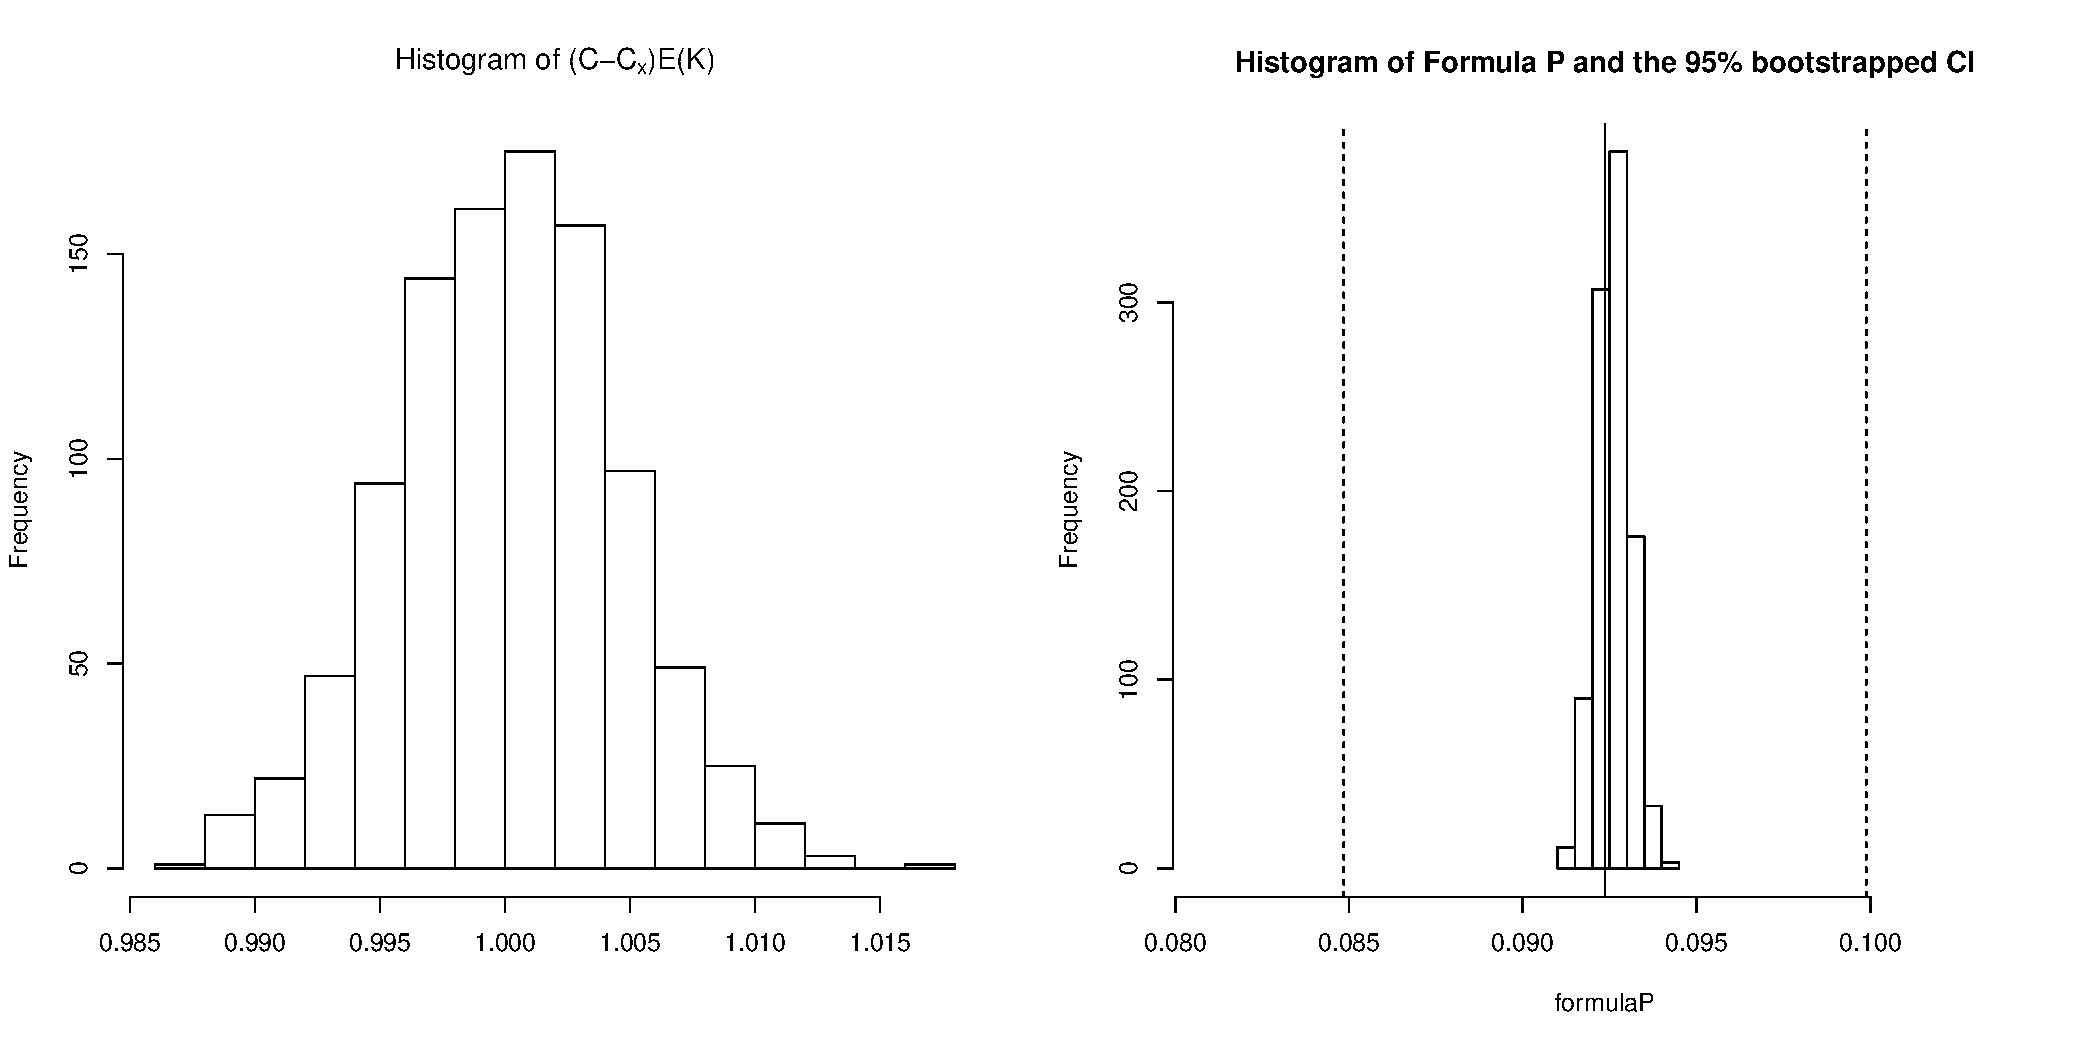
\includegraphics[width=\textwidth]{kpois6}
  \caption{Left: Histogram of $(\wht{C}-\wht{C_x})\wht{\bbe K_i^{(r)}}$. Right: Histogram of the $1000$ estimates from Formula P and the 95\% confidence interval form bootstrap. The two dashed lines are lower and upper bound of the confidence interval and the solid line is the sample variance of $1000$ realization of $\xbar_1-\xbar_2$ multiplied by $n$}
  \label{fig:kpois6}
\end{figure}
We first use $Poisson(6)$ to generate $K_i$, and then $K_i^{(r)},r=1,2$ from the binomial distribution. The left plot in Figure \ref{fig:kpois6} shows that $C-C_x$ is indeed close to $1/\bbe K_i^{(r)}$. The ratio of the two is normally distributed and concentrated around 1. The right plot shows all the $1000$ estimates from Formula P are within the bootstrpped confidence interval. 



%A similar simulation was done for Poisson(6) distribution. Figure~\ref{fig:kpois6} shows the performance of \ref{p_est}. 
%\begin{figure}[!htp]
%  \centering
%  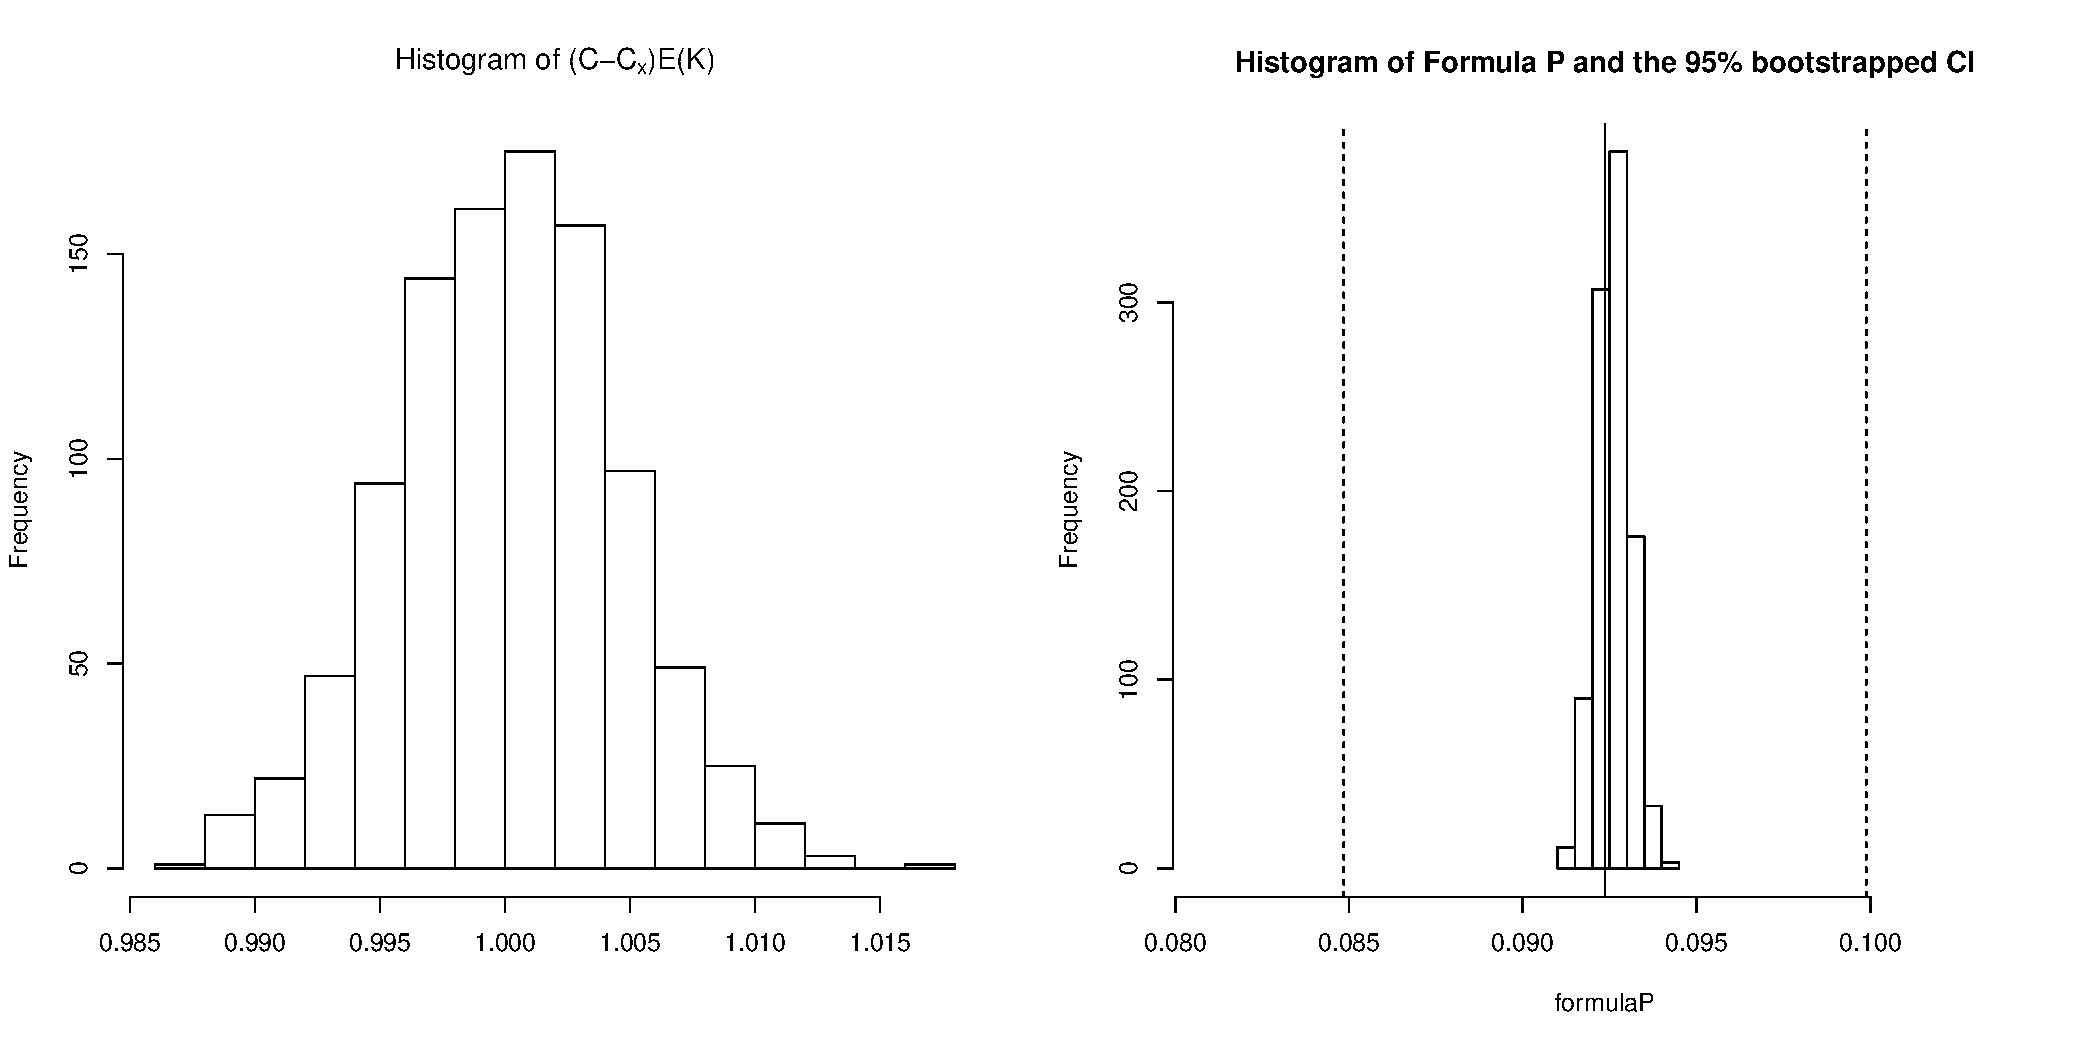
\includegraphics[width=0.5\textwidth]{kpois6}
%  \caption{Histogram of the $1000$ estimates from Formula P and the 95\% confidence interval form bootstrap. The two dashed lines are lower and upper bound of the confidence interval and the solid line is the sample variance of $1000$ realization of $\xbar_1-\xbar_2$ multiplied by $n$}. 
%  \label{fig:kpois6}
%\end{figure}
%\clearpage
\subsection{$K_i$ constant case}
In this simulation study, we fixed $K_1=5$. Figure~\ref{fig:kfixed5} shows the performance in this case.

\begin{figure}[!hbtp]
  \centering
  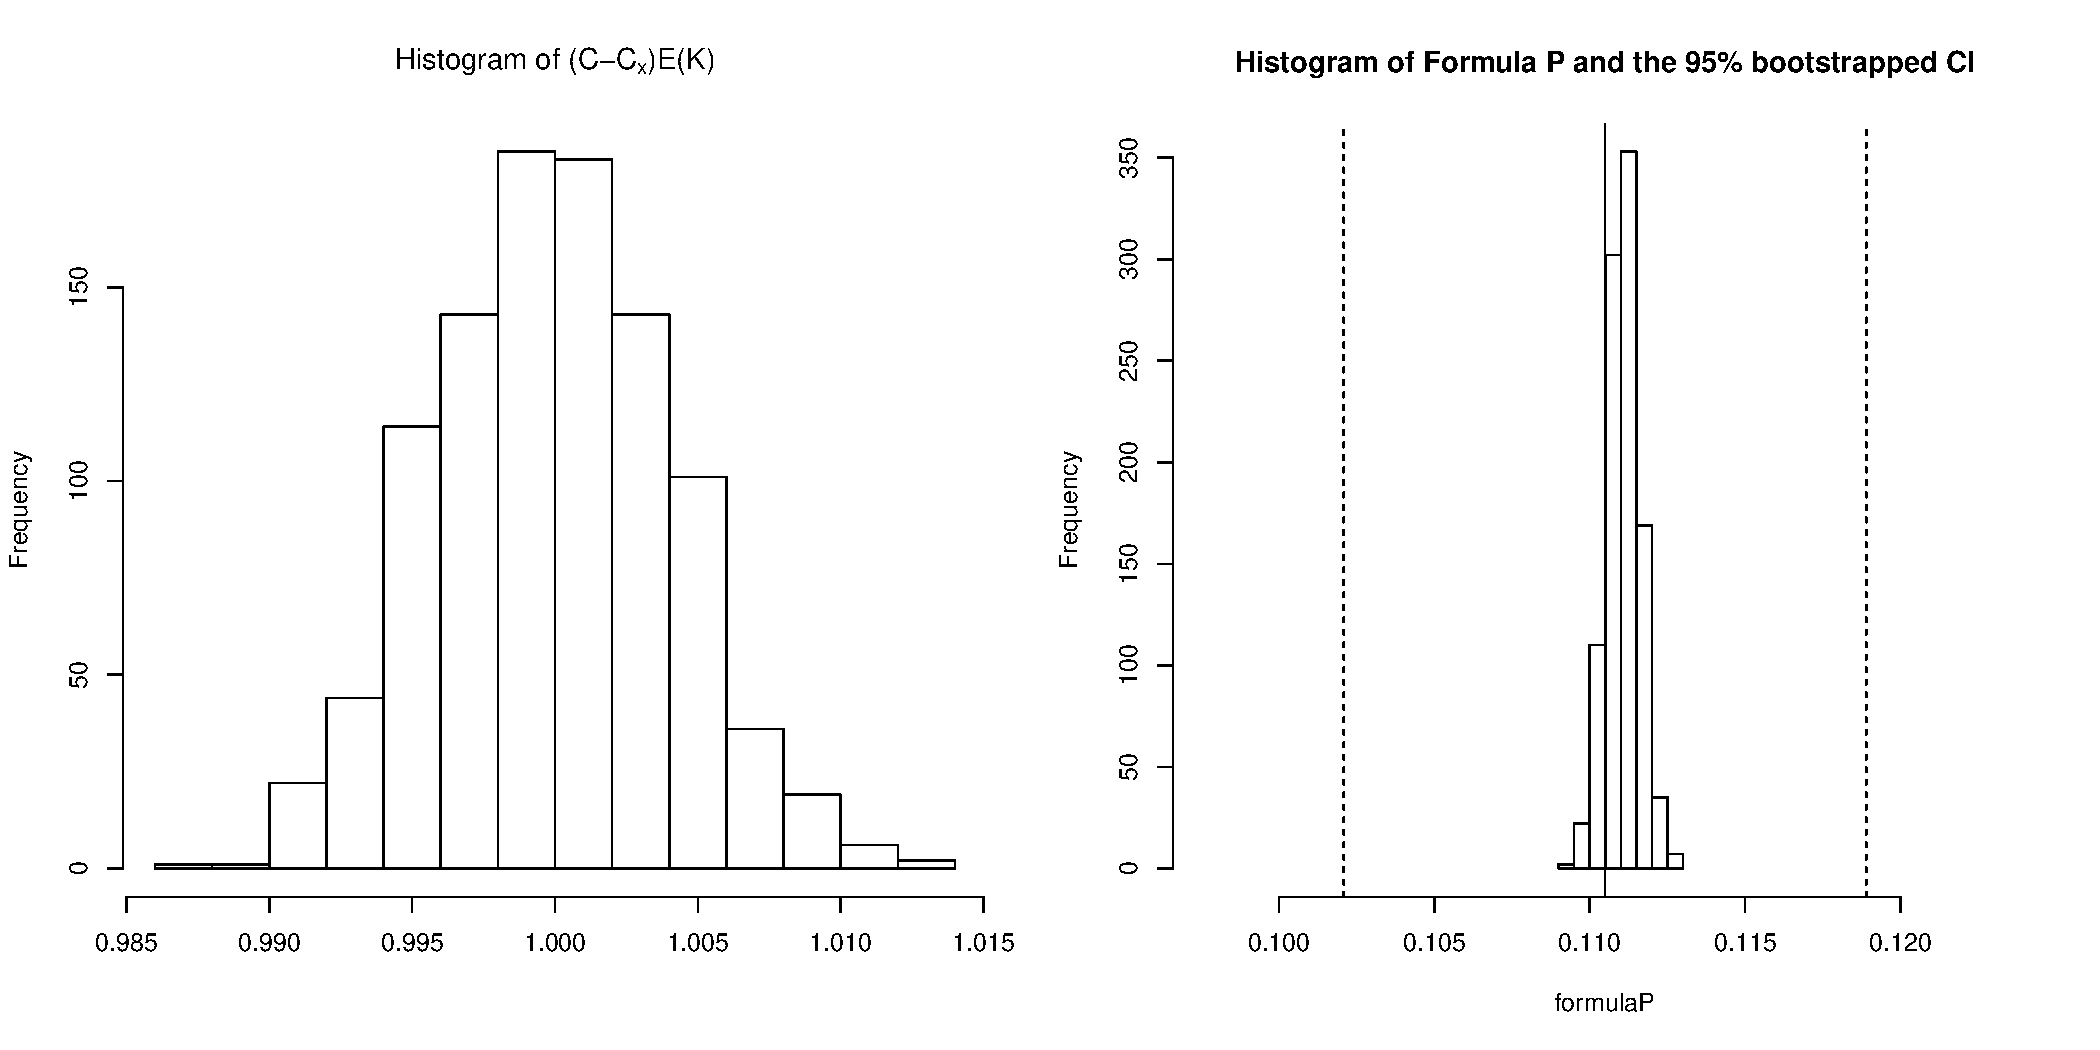
\includegraphics[width=\textwidth]{kfixed5}
    \caption{Left: Histogram of $(\wht{C}-\wht{C_x})\wht{\bbe K_i^{(r)}}$. Right: Histogram of the $1000$ estimates from Formula P and the 95\% confidence interval form bootstrap. The two dashed lines are lower and upper bound of the confidence interval and the solid line is the sample variance of $1000$ realization of $\xbar_1-\xbar_2$ multiplied by $n$}
  \label{fig:kfixed5}
\end{figure}

%\begin{figure}[!hbtp]
%  \centering
%  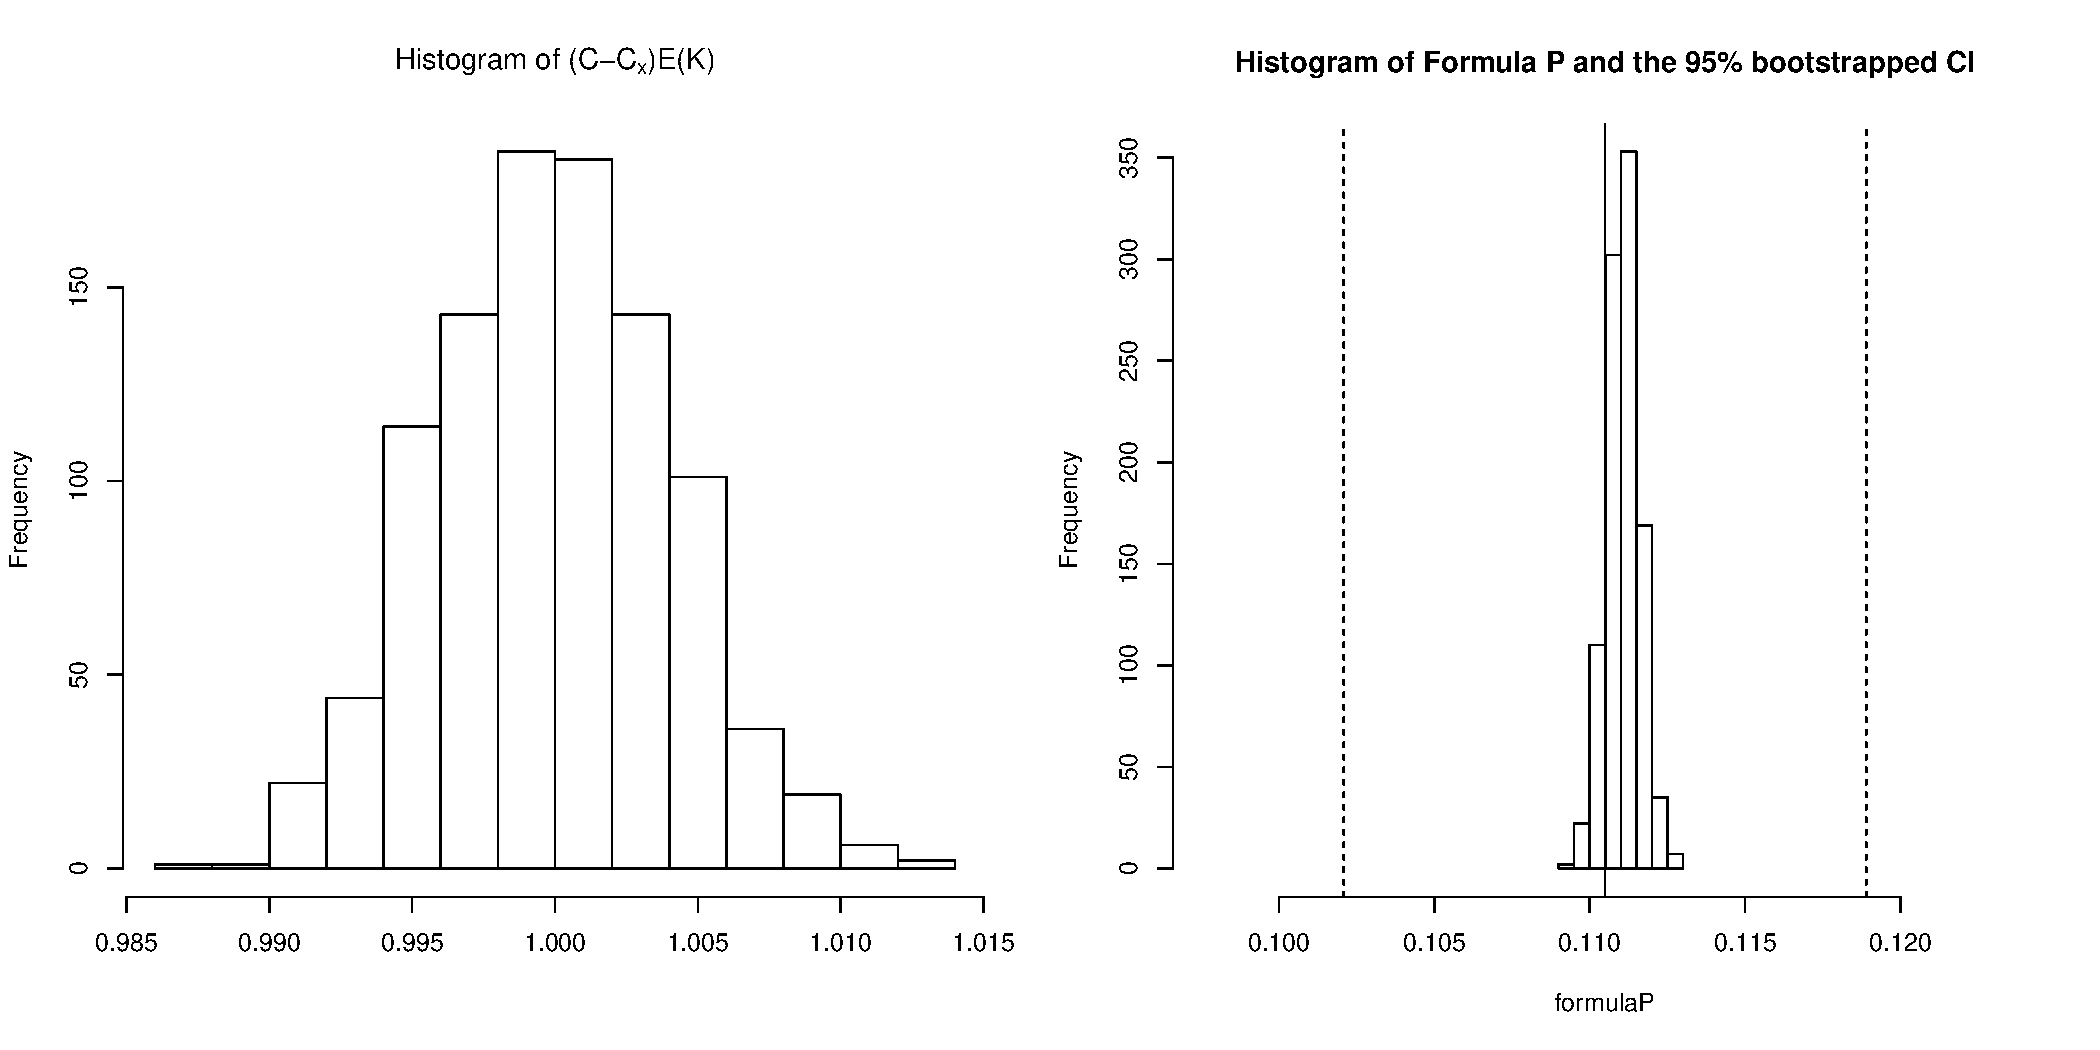
\includegraphics[width=0.5\textwidth]{kfixed5}
%  \caption{Histogram of the $1000$ estimates from Formula P and the 95\% confidence interval form bootstrap. The two dashed lines are lower and upper bound of the confidence interval and the solid line is the sample variance of $1000$ realization of $\xbar_1-\xbar_2$ multiplied by $n$}. 
%  \label{fig:kfixed5}
%\end{figure}
%Figure ~\ref{fig:kfixed5} shows the performance of Formula N in this case. 

\appendix
\section{Assumption Check}
In this appendix, we do an empirical check of the assumption that $K_i$ and $(\mu_i, \sigma_i^2)$ is independent. In particular, we will estimate $cor(K_i, \mu_i)$ using data collected from some control flight. Data was collected for FLT-ONE-CF1 and FLT-TWO-CF2 on 4/1/2011. The page view level metrics under examination is: \emph{PLT, logPLT, overall PCR, Ad PCR, Answer PCR, Ad Clicks}. For each user, $\mu_i$ --- the mean of the page level measurement was estimated simply by corresponding sample mean. The results are organized in the following table.
\begin{center}
   \begin{tabular}{| c|c| c| c| c | c |}
\hline
   PLT & logPLT& overallPCR& AdPCR& AnswerPCR& AdClicks\\
  \hline
 $-0.054$& $-0.100$&$-0.016$&$-0.019$&$-0.004$&$-0.016$\\
     \hline
   \end{tabular}
 \end{center}

All correlation is low. logPLT has the largest absolute value, and it suggests (and also intuitively true) that PLT should affect user's visit frequency negatively. But this effect is still low overall.  

\end{document}